\section{Comparison}
    These are our results during 100 cycles. In the comparison, difference between the simulation results and the actual change in fine dust concentration is recognizable. In the simulation results, the boundary of fine dust concentration gradually breaks down and spreads, while the actual fine dust maintains the boundary and shifts together.
    \begin{figure}[htb!]
        \centering
        \begin{tabular}{cc}
            \subfloat[cycle 1]{{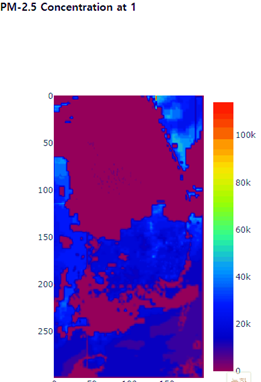
\includegraphics[scale=1.2]{cycle1.png}}}&
            \subfloat[cycle 21]{{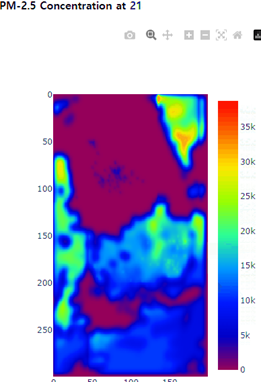
\includegraphics[scale=1.2]{cycle21.png}}}\\
            \subfloat[cycle 51]{{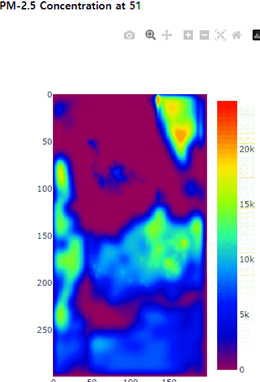
\includegraphics[scale=1.2]{cycle51.png}}}&
            \subfloat[cycle 91]{{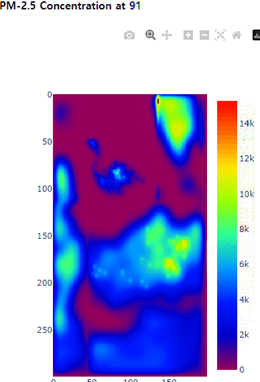
\includegraphics[scale=1.2]{cycle91.png}}}\\
        \end{tabular}
        \caption{The simulation results during 100 cycles}
    \end{figure}\clearpage
    \begin{figure}[htb!]
        \centering
        \begin{tabular}{cc}
            \subfloat[11:45]{{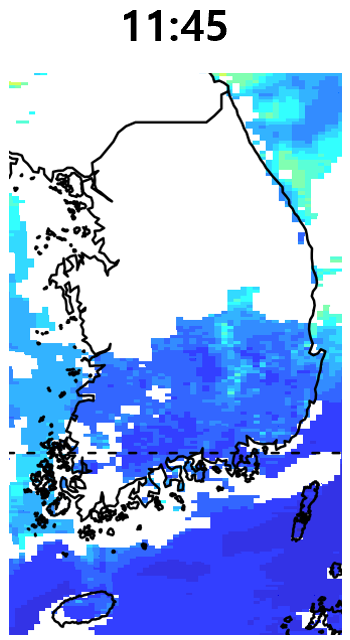
\includegraphics[scale=0.6]{1145.png}}}&
            \subfloat[12:45]{{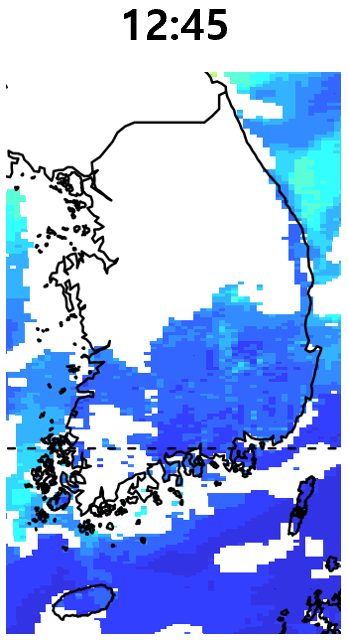
\includegraphics[scale=0.6]{1245.png}}}\\
            \subfloat[13:45]{{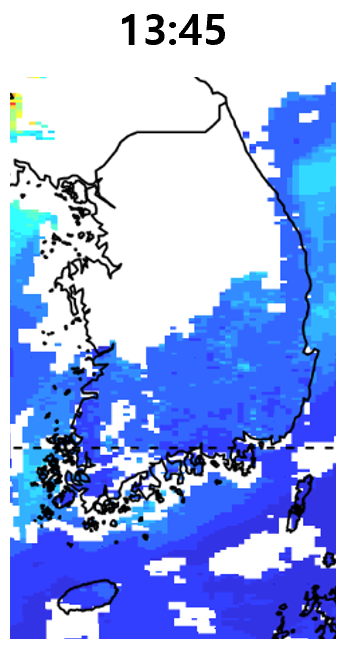
\includegraphics[scale=0.6]{1345.png}}}&
            \subfloat[14:45]{{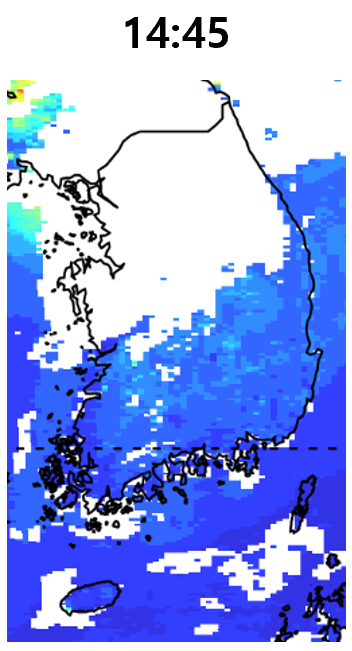
\includegraphics[scale=0.6]{1445.png}}}\\
        \end{tabular}
        \caption{The real data on Nov 01, 2023}
    \end{figure}